% example with several commonly used tex constructs
\section{Concept}
% define a marker to be referenced from outside:
\hyperdef{dtor}{concept}{[Marker:dtor.concept]}\\
As mentioned in the introduction, there are several scenarios or
use cases for the \DDA~ reflecting differing requirements and
delivery dates.
\subsection{\DDA~ use cases}
\index{Demonstrator!use cases}
\subsubsection{Detector test bed}
Detector tests with a free running system are needed to verify
that the data rates are not very much bigger than expected (dark
noise).
\subsubsection{Switched event building}
Independent of the data sources (\ABB~ or GigabitEthernet) several mechanisms for the switched
event building must be implemented and tested.
\subsubsection{DAQ framework and control systems}
There are still several options for the choice of the control system. The \xdaq~ framework
provides several communication mechanisms. The control system not necessarily must be \xdaq~ but
could be e.g. EPICS based. In such a case gateways must be implemented.
\subsubsection{\mbs~ replacement}
\index{Demonstrator!MBS} Very probably there will be no complete
replacement of the \mbs~ possible for the next years. A very big
amount of existing hardware of running \mbs~ systems cannot be
replaced neither they can be attached directly to the new DAQ
framework. At least the effort to replace the software running on
the front-end CPUs (RIO, Lynx, \mbs~) would be too big, if
possible. Instead one could envision that the \mbs~ front-end
nodes, i.e. the readout nodes, send their sub-event data peer to
peer to new event builder nodes (new \mbs~ mode). Each of these
nodes functions as sub-event receiver (Ethernet, TCP) and sends
the data for event building through the data transport network
like InfiniBand to the others and functions also as event
processor. The Ethernet input channel replaces the \ABB~input
channel.
\subsubsection{Hybrid setup}
If the system should run in production, very probably a hybrid of
\mbs~ for ancillary components and new front ends will be needed.
When running in triggered mode, the trigger of the new components
must be synchronized with the \mbs~ trigger system. In triggerless
mode the \mbs~ data must be time stamped or \mbs~ triggers must be
injected and recorded in one of the time stamped data streams by
connecting the trigger bus directly to an \FEB.
\subsubsection{Front end test bed}
The new components \FEB, \DCB, and \ABB~and their connections must be tested.
The timing system and the triggered/non-triggered mode must be tested.

\subsection{The name}
Because the systems described might be also used by other
experiments it might evolve to more than a demonstrator. At the
other hand it will not provide components of the front-end side
but rather provide the hooks and plug-ins to attach a big variety
of front-end systems and components. There is one principal
restriction, however, in the current design. There is nothing like
a 2nd level trigger. That means, that we assume that the full data
rate can be switched through a network for event building.
However, a congestion prevention must be provided generating dead
time for the detector readout. From this point on we have only
event filters. The front-ends might however be triggered or free
running.

The demonstrator as a production system would be rather a backbone. Therefore we propose a name like\\
Data Acquisition Backbone Framework {\bf DBF} (DataBaseFormat!) or {\bf ABF}\\
Data Acquisition Backbone System {\bf DBS} (Deutscher Bildungs-Server) or {\bf ABS}\\
Data Acquisition Backbone Core {\bf DABC} or {\bf ABC}\\
FAIR Acquisition Backbone {\bf FAB}

\section{\dabc~ architecture}
\begin{figure}[htb]
\centering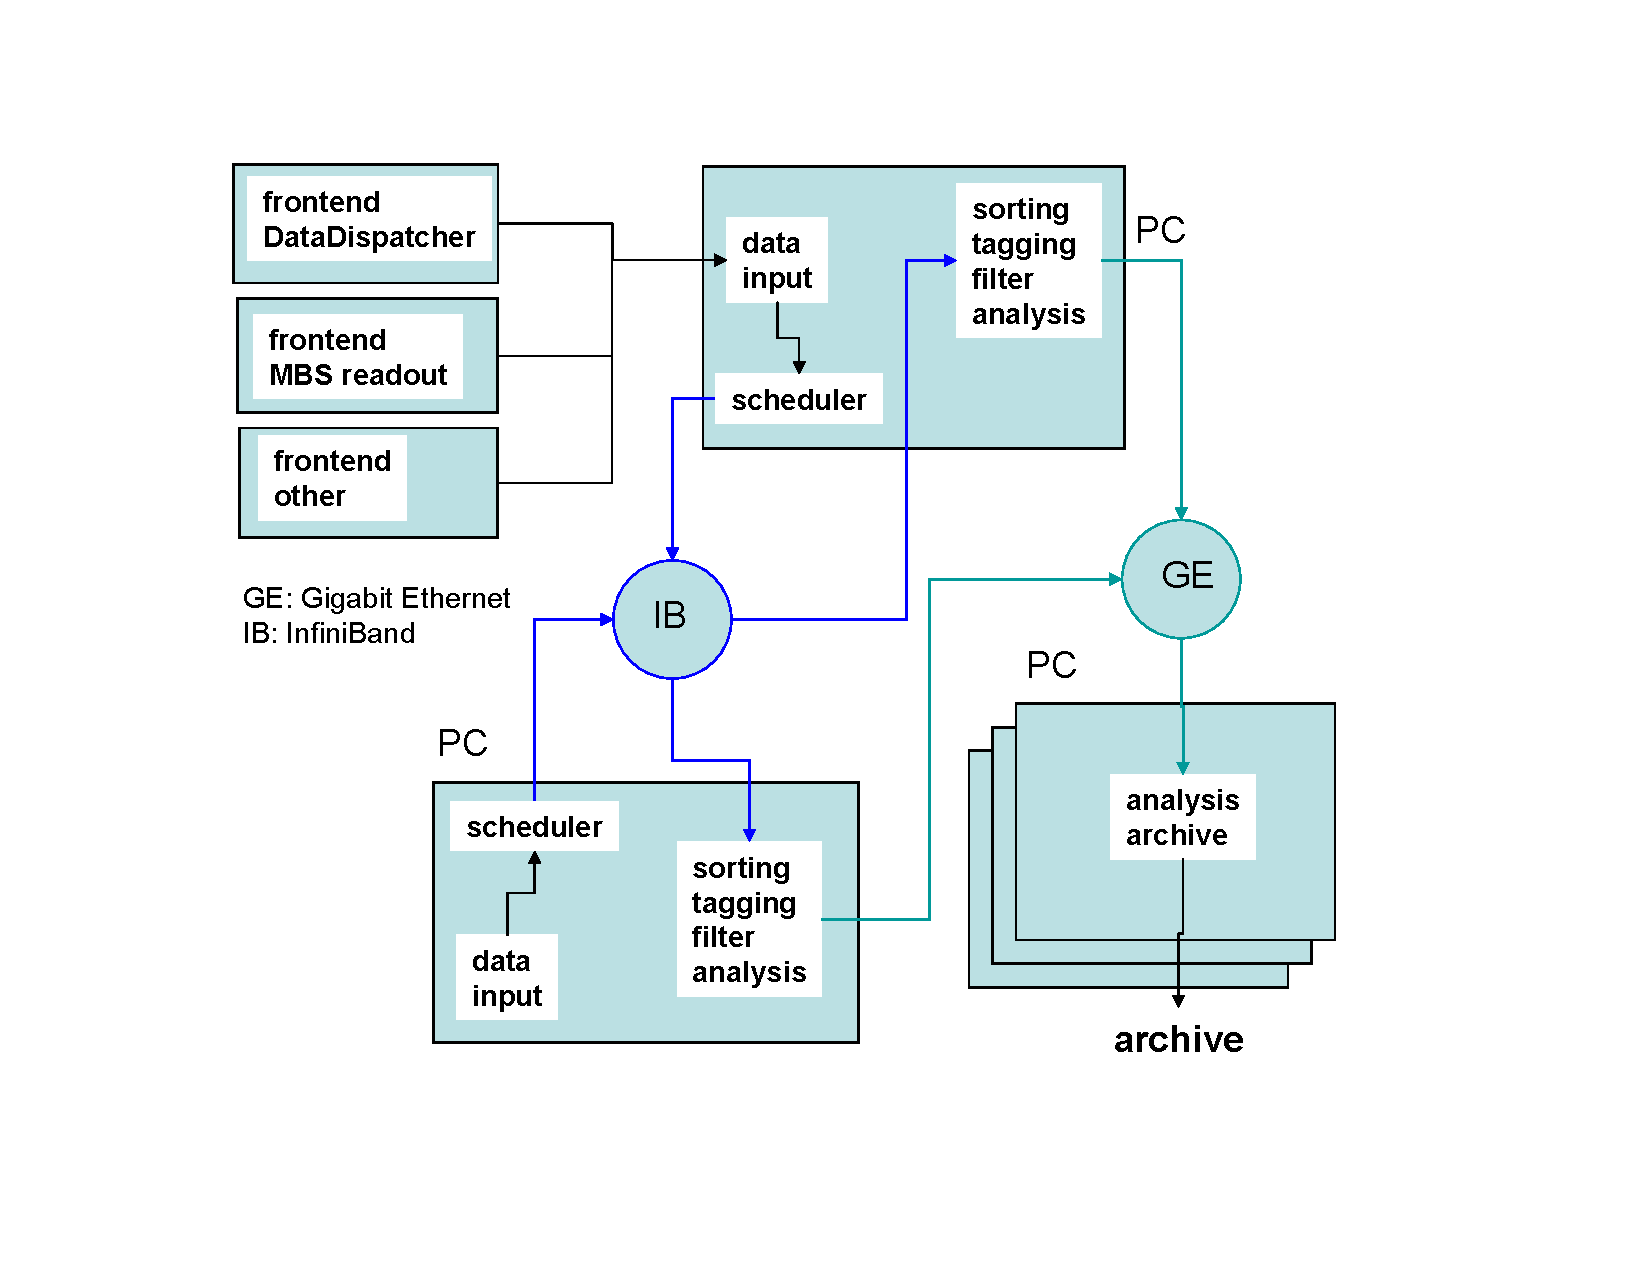
\includegraphics[width=.8\textwidth] {dtor_sw-over_4}
\caption{\dabc~ data flow and components}
\label{fig:dtor_sw-over_4}
\end{figure}

\section{Implementation phases}
One can identify four implementation phases, i.e. time scales:
\begin{compactenum}
\item \mbs~ front end support
\item Hardware tests and basic functionality of framework
\item Detector test
\item Production system
\end{compactenum}
Phase 0 might be in the beginning necessary for elementary test of the boards and the data links.
The software of phase 0 will be "experimental" and not part of the system.
\section{Requirements}
\subsection{Frontend test bed}
Phase 0, 1
\begin{figure}[htb]
\centering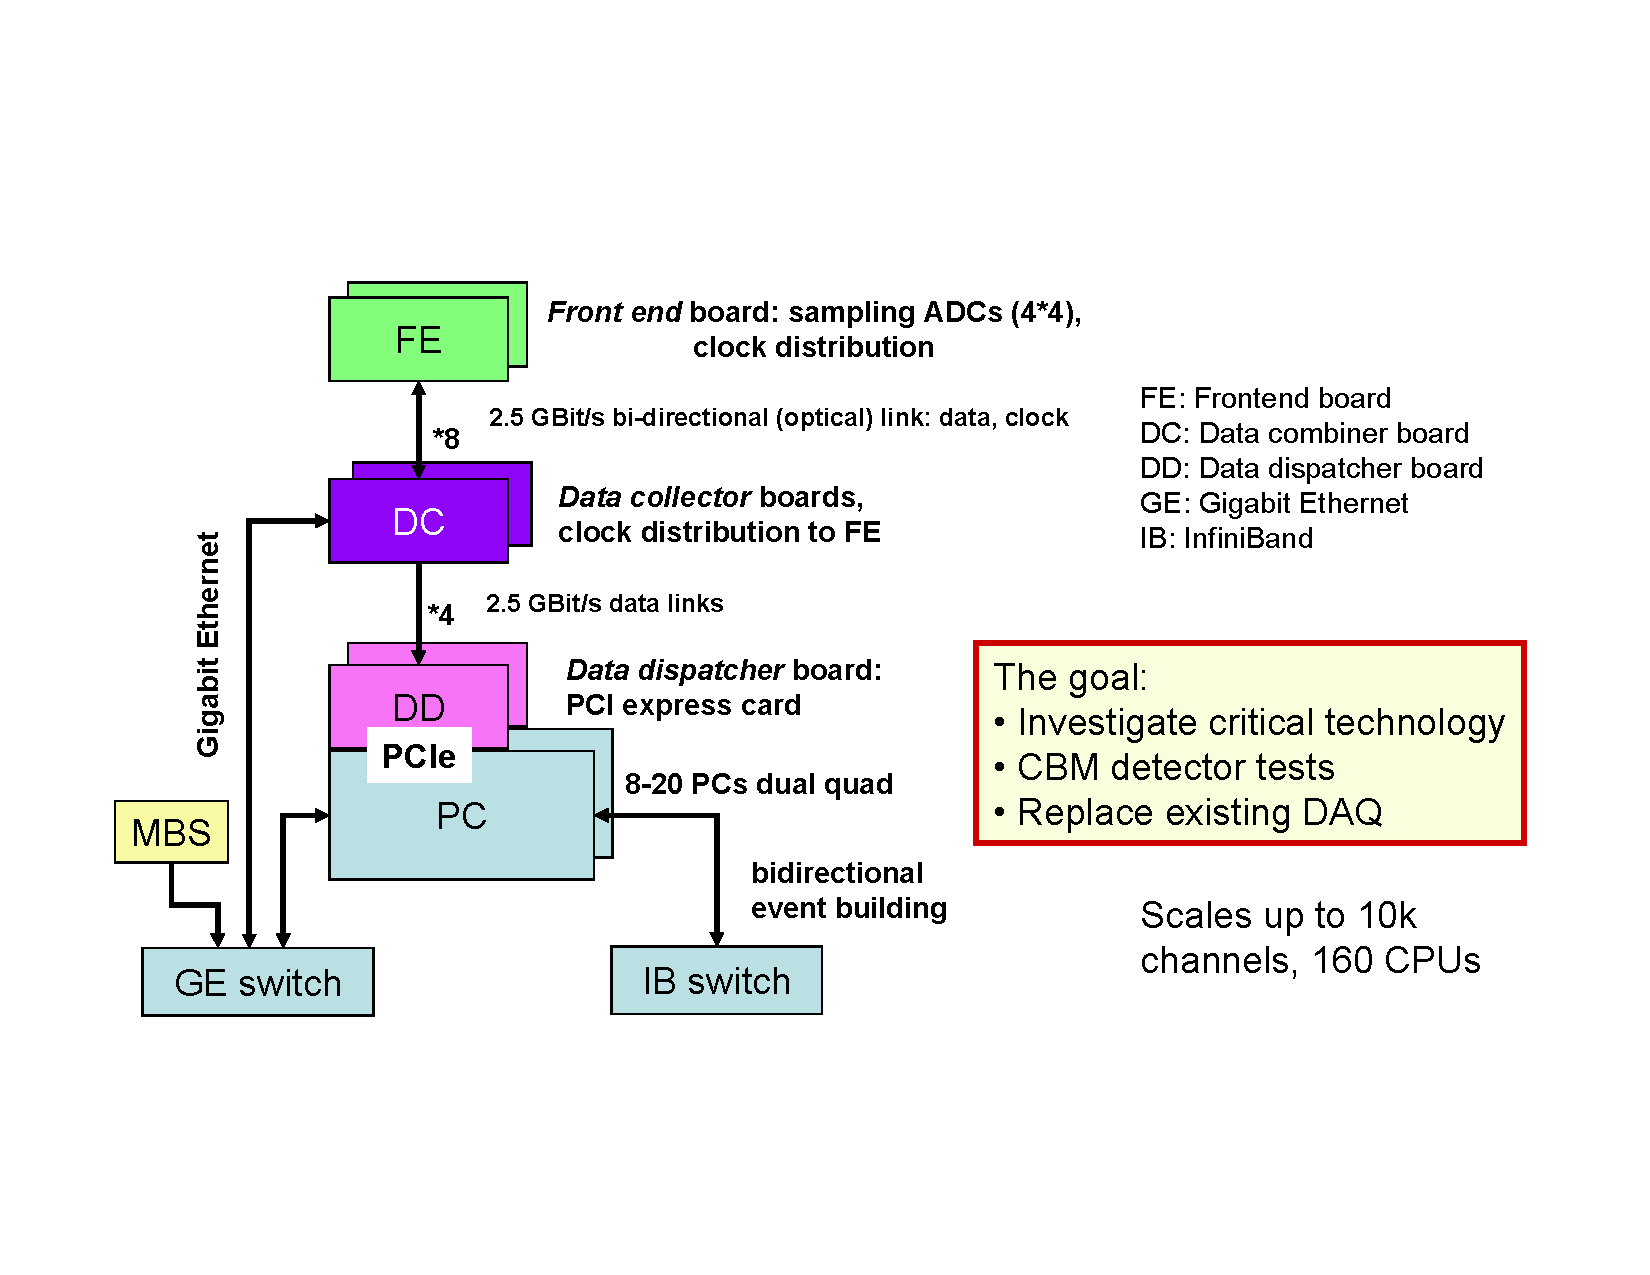
\includegraphics[width=.8\textwidth] {demof-all}
\caption{\dabc~ overall data processing architecture}
\label{fig:dtor-daq-over}
\end{figure}

\begin{figure}[htb]
\centering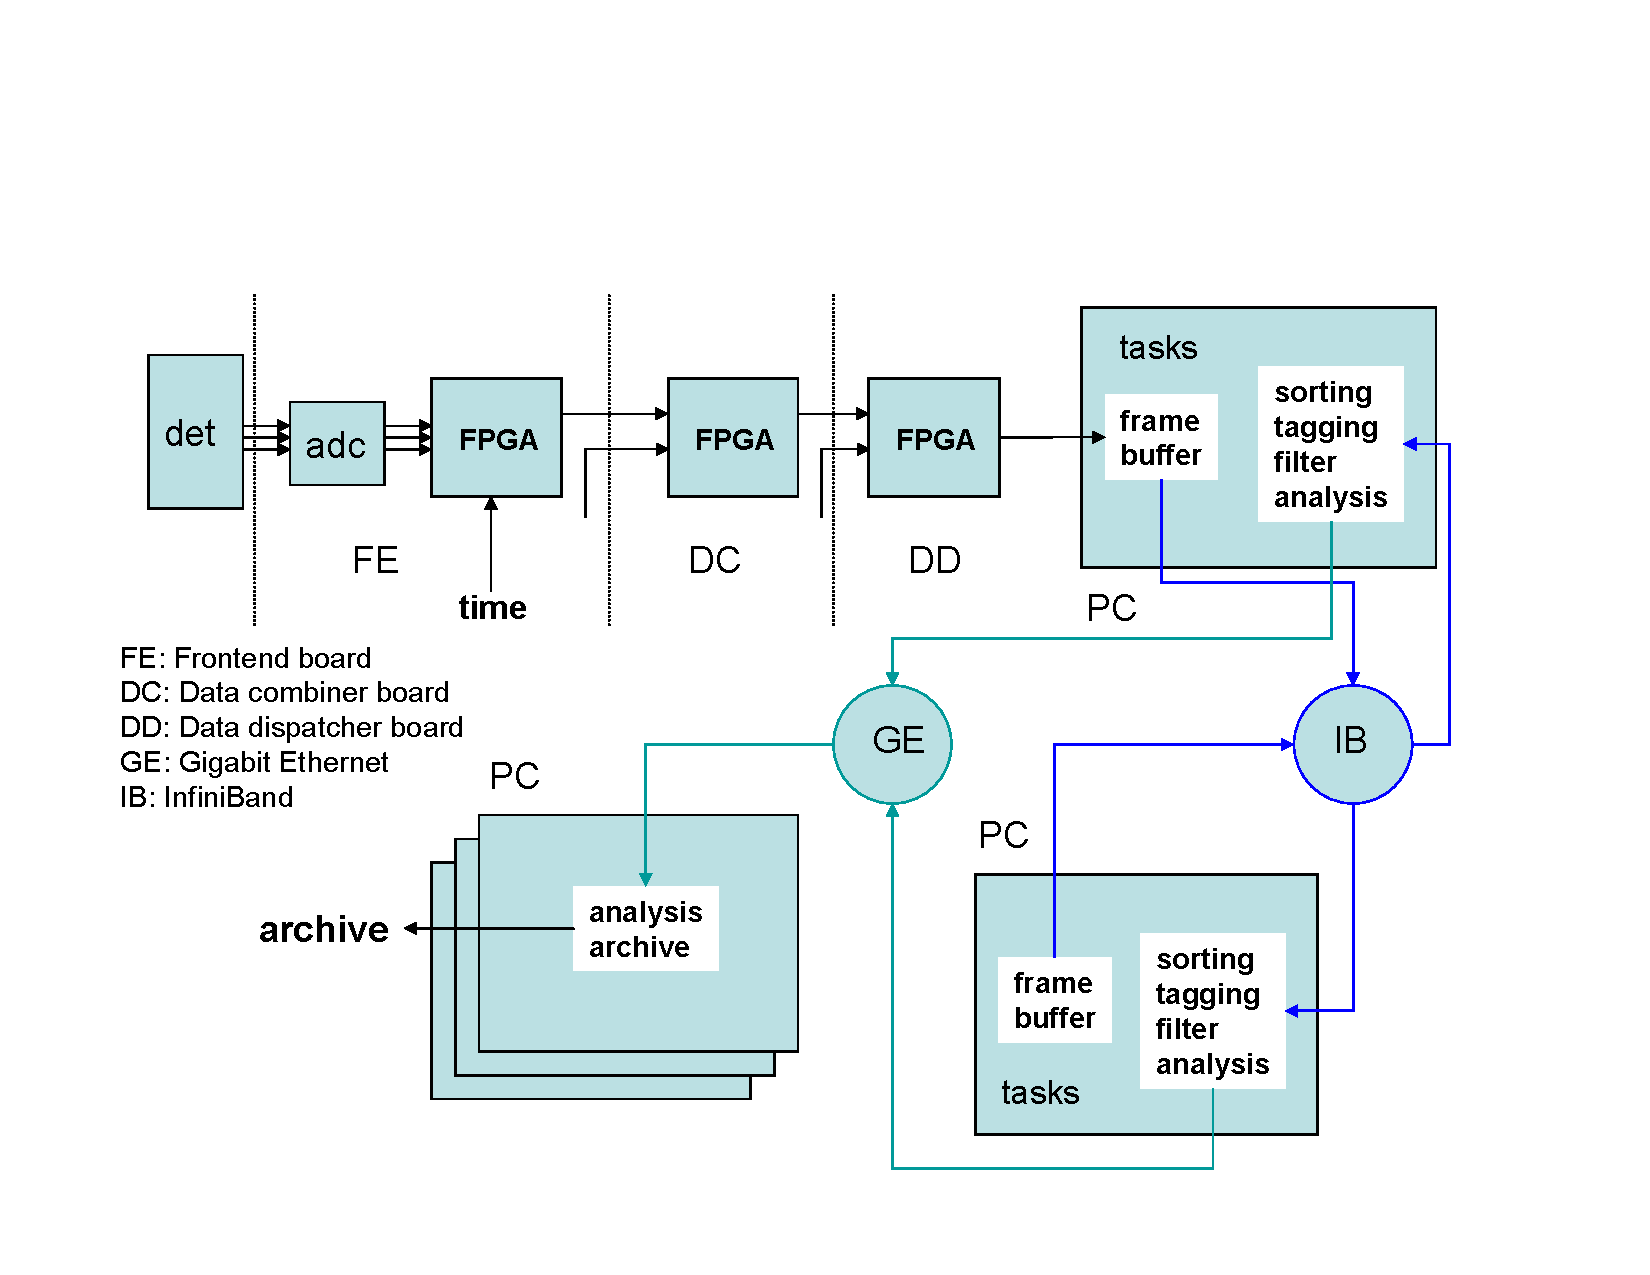
\includegraphics[width=.8\textwidth]{sw-over} % pdf file
\caption{Overall data streams architecture}
\label{fig:dtor-struct-over} % give it a name for references
\end{figure}

Fig.~\ref{fig:dtor-daq-over} shows the hardware components,
fig.~\ref{fig:dtor-struct-over} shows the data streams.
\subsection{Detector test bed}
Phase 2
\subsection{Switched event building}
Phase 2
\subsection{DAQ framework and control systems}
Phase 2
\subsection{\mbs~ front-end support}
Phase 1
\subsection{Hybrid setup}
Phase 4
